\documentclass[11pt,a4paper]{article}

\usepackage[margin=2.3cm]{geometry}
\usepackage[T1]{fontenc}
\usepackage{lmodern}
\usepackage{amsmath}
\usepackage{graphicx}
\usepackage{booktabs}
\usepackage{float}
\usepackage{caption}
\usepackage{xcolor}
\usepackage{listings}
\usepackage{tikz}
\usetikzlibrary{arrows.meta,positioning,calc,fit}
\usepackage[colorlinks=true,linkcolor=blue!50!black,urlcolor=blue!50!black]{hyperref}

\captionsetup{font=small,labelfont=bf}
\setlength{\parskip}{4pt}
\setlength{\parindent}{0pt}

\definecolor{codebg}{RGB}{246,246,246}
\lstset{basicstyle=\ttfamily\footnotesize,backgroundcolor=\color{codebg},frame=single,
        rulecolor=\color{black!20},breaklines=true,columns=fullflexible,keepspaces=true,
        keywordstyle=\color{blue!60!black},commentstyle=\color{green!40!black},language=Python,
        xleftmargin=4pt,xrightmargin=4pt}

\tikzset{
  box/.style={draw,rounded corners=2pt,align=center,font=\small,minimum height=9mm,inner sep=4pt},
  arr/.style={-{Stealth[length=2.2mm]},thick}
}

\begin{document}

% ------------------------------------------------------------------ cover
\begin{titlepage}
\centering
\vspace*{2.5cm}
{\large Egypt-Japan University of Science and Technology (E-JUST)\par}
\vspace{0.3cm}
{\large Deep Learning --- Project 1\par}
\vspace{2.5cm}
{\LARGE\bfseries Frame-Level Phoneme Recognition\\[4pt] with a Multilayer Perceptron\par}
\vspace{0.6cm}
{\large Kaggle competition 11-785 HW1P2 (Fall 2024)\par}
\vspace{3cm}
{\large\bfseries Yassin Mahmoud Alam Elden Abdelaziz\par}
\vspace{0.2cm}
{\large ID: 120230122\par}
\vfill
{\large November 2026\par}
\end{titlepage}

\tableofcontents
\vspace{0.6cm}

\begin{center}
\fbox{\begin{minipage}{0.9\textwidth}
\textbf{Results at a glance.}
Final model: 6-hidden-layer MLP, \textbf{10,519,592 parameters} (limit: 20M), input of 41 frames
$\times$ 28 MFCCs. \textbf{Dev accuracy 84.55\%} (best epoch 19 of 20), train accuracy 86.81\%,
dev loss 0.471. The ablation study raised dev accuracy from 68.06\% (baseline) to 82.90\% in seven
steps of 3 epochs each. Training time: about 42 min for the ablation study and 67.6 min for the final
model, on one RTX~4050 Laptop GPU (6 GB).
\end{minipage}}
\end{center}

\newpage
% ------------------------------------------------------------------ 1
\section{Goal of the project}

Speech is recorded as a sound wave and cut into short \emph{frames} of 10\,ms. Each frame is described by
28 \emph{MFCC} numbers (Mel-Frequency Cepstral Coefficients, a compact description of the sound's
frequency content). The task is to predict, \textbf{for every single frame}, which of \textbf{40 phoneme
classes} is being spoken: 39 English phonemes (ARPAbet) plus silence \texttt{[SIL]}.

The goals of the project were:
\begin{enumerate}\itemsep0pt
  \item Build a \textbf{multilayer perceptron (MLP)} classifier (no CNNs or RNNs) with fewer than
        \textbf{20 million parameters}.
  \item Reach a high frame accuracy on the hidden test set and submit the predictions to Kaggle as
        \texttt{submission.csv}.
  \item Show \textbf{why} each design choice was made, using an ablation study.
  \item Keep the code \textbf{simple and explainable}: plain PyTorch, one model class, one training loop.
\end{enumerate}

The metric is \textbf{accuracy}: the share of test frames whose predicted phoneme is correct.

% ------------------------------------------------------------------ 2
\section{Dataset}

The data comes from LibriSpeech (read English audiobooks). Each recording is one \texttt{.npy} file of
shape $(T, 28)$ ($T$ = number of frames). Its transcript has one phoneme per frame, plus a
\texttt{[SOS]} and an \texttt{[EOS]} token that we remove because they do not match any frame.

\begin{table}[H]
\centering
\begin{tabular}{lrrl}
\toprule
Split & Recordings & Frames & Use \\
\midrule
\texttt{train-clean-100} & 28,539 & 36,091,157 & training \\
\texttt{dev-clean}       &  2,703 &  1,928,204 & validation (model and setting selection) \\
\texttt{test-clean}      &  2,620 &  1,934,138 & final predictions (labels hidden) \\
\bottomrule
\end{tabular}
\caption{Dataset splits.}
\end{table}

\begin{figure}[H]
\centering
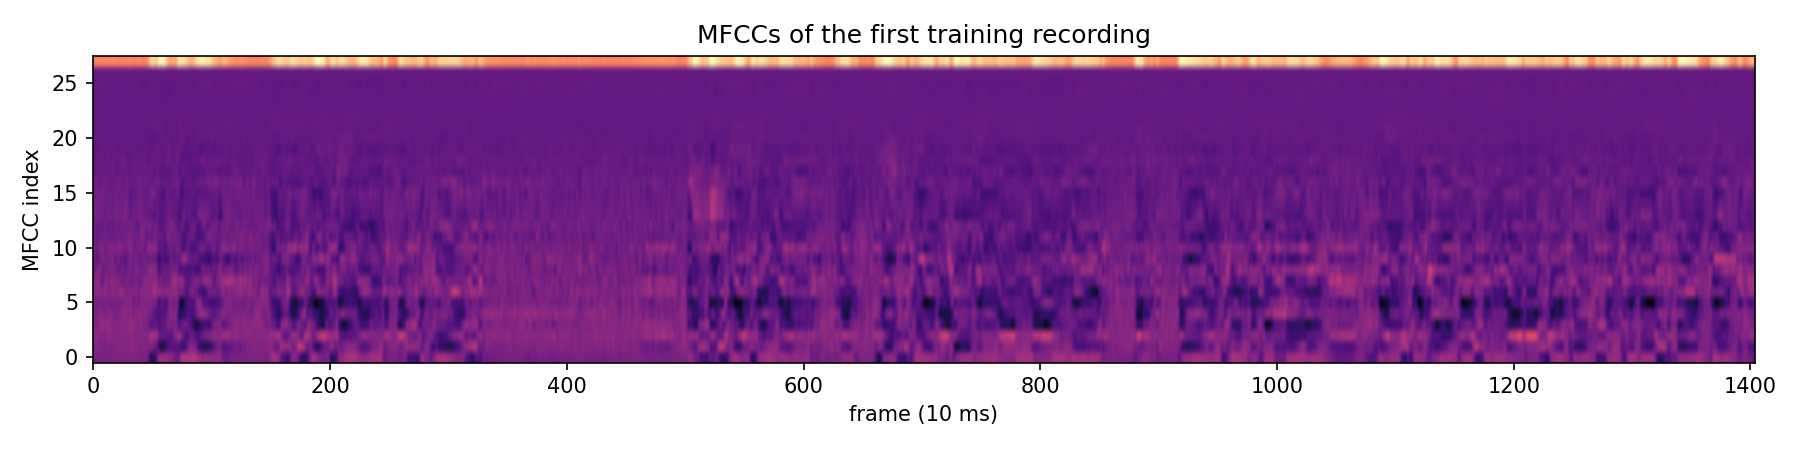
\includegraphics[width=0.95\textwidth]{figures/mfcc_example.png}
\caption{The 28 MFCCs of one training recording (x-axis: time in frames, y-axis: coefficient).}
\end{figure}

\begin{figure}[H]
\centering
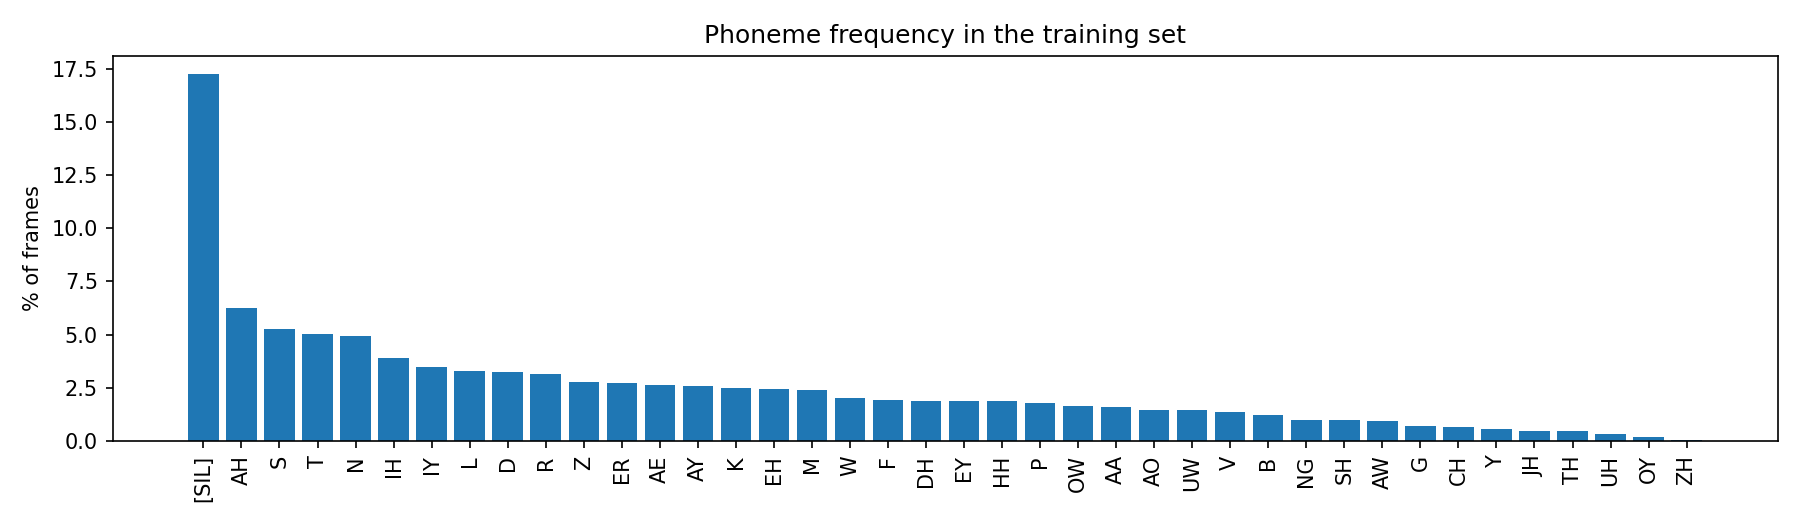
\includegraphics[width=0.95\textwidth]{figures/class_distribution.png}
\caption{Phoneme frequency in the training set. The classes are imbalanced: \texttt{[SIL]} is 17.3\% of
the frames, and the rarest phoneme (\texttt{ZH}) is under 0.1\%.}
\label{fig:classes}
\end{figure}

Because of this imbalance, always predicting \texttt{[SIL]} would already give about 16.6\% accuracy on
dev. Every model must clearly beat this trivial level, and we also check per-phoneme accuracy
(Section~\ref{sec:errors}), not only overall accuracy.

% ------------------------------------------------------------------ 3
\section{Workflow}

\begin{figure}[H]
\centering
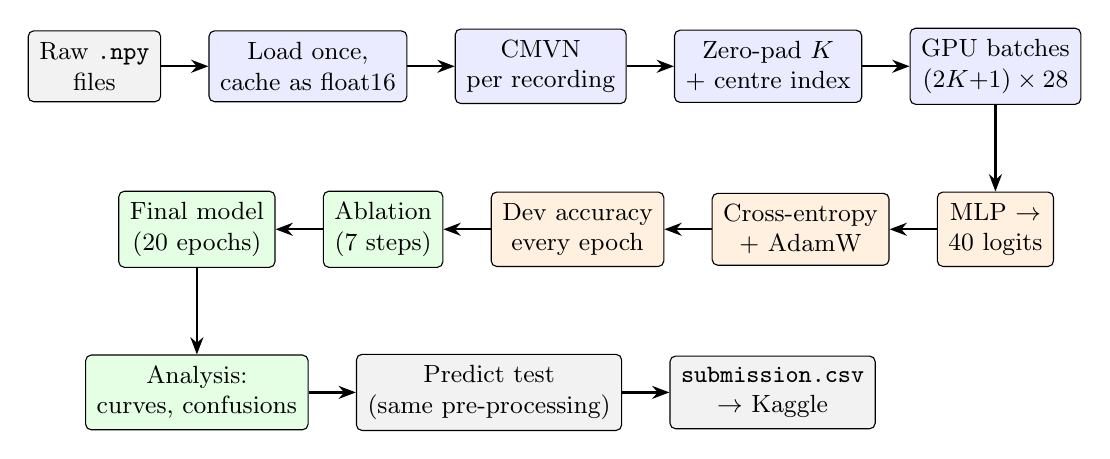
\begin{tikzpicture}[node distance=5mm and 6mm]
  \node[box,fill=gray!10]  (raw)   {Raw \texttt{.npy}\\files};
  \node[box,fill=blue!8,right=of raw]   (load)  {Load once,\\cache as float16};
  \node[box,fill=blue!8,right=of load]  (cmvn)  {CMVN\\per recording};
  \node[box,fill=blue!8,right=of cmvn]  (pad)   {Zero-pad $K$\\+ centre index};
  \node[box,fill=blue!8,right=of pad]   (batch) {GPU batches\\$(2K{+}1)\times28$};

  \node[box,fill=orange!12,below=11mm of batch] (mlp)  {MLP $\rightarrow$\\40 logits};
  \node[box,fill=orange!12,left=of mlp]  (train) {Cross-entropy\\+ AdamW};
  \node[box,fill=orange!12,left=of train] (dev)  {Dev accuracy\\every epoch};
  \node[box,fill=green!10,left=of dev]   (abl)  {Ablation\\(7 steps)};
  \node[box,fill=green!10,left=of abl]   (fin)  {Final model\\(20 epochs)};

  \node[box,fill=green!10,below=11mm of fin]  (ana)  {Analysis:\\curves, confusions};
  \node[box,fill=gray!10,right=of ana]   (test) {Predict test\\(same pre-processing)};
  \node[box,fill=gray!10,right=of test]  (sub)  {\texttt{submission.csv}\\$\rightarrow$ Kaggle};

  \draw[arr] (raw)--(load); \draw[arr] (load)--(cmvn); \draw[arr] (cmvn)--(pad); \draw[arr] (pad)--(batch);
  \draw[arr] (batch)--(mlp); \draw[arr] (mlp)--(train); \draw[arr] (train)--(dev); \draw[arr] (dev)--(abl);
  \draw[arr] (abl)--(fin); \draw[arr] (fin)--(ana); \draw[arr] (ana)--(test); \draw[arr] (test)--(sub);
\end{tikzpicture}
\caption{The complete workflow. Blue: data pipeline. Orange: one training run. Green: experiments.
Grey: input and output.}
\label{fig:workflow}
\end{figure}

\begin{enumerate}\itemsep0pt
  \item \textbf{Check the GPU} and stop with an error if it is missing (training on a CPU would take days).
  \item \textbf{Load and cache the data}: all recordings of a split are merged into one array and saved to
        \texttt{cache/} (Section~\ref{sec:loading}).
  \item \textbf{Pre-process}: CMVN normalisation and context padding (Sections~\ref{sec:cmvn}--\ref{sec:context}).
  \item \textbf{Sanity check}: the model must be able to memorise a single batch (Section~\ref{sec:sanity}).
  \item \textbf{Ablation study}: add one improvement at a time and measure it (Section~\ref{sec:ablation}).
  \item \textbf{Final training}: train the best configuration for 20 epochs (Section~\ref{sec:final}).
  \item \textbf{Analyse} errors and \textbf{predict} the test set to create \texttt{submission.csv}.
\end{enumerate}

Before the real run, the whole notebook was tested end to end in \texttt{DEBUG} mode (500 training
recordings, 1--2 epochs) to catch bugs in minutes instead of hours.

% ------------------------------------------------------------------ 4
\section{Method}

\subsection{Loading and caching the data}\label{sec:loading}
Reading about 34,000 small files is slow, so each split is read \textbf{once} and saved as one
\texttt{.npz} file holding three arrays:
\begin{itemize}\itemsep0pt
  \item \texttt{feats} $(N_\text{frames}, 28)$: all recordings stacked, stored as \textbf{float16} (2\,GB
        instead of 4\,GB for train; MFCCs do not need more precision);
  \item \texttt{lens}: the number of frames in each recording, so we know where each one starts and ends;
  \item \texttt{labels}: one class index per frame, as \texttt{uint8} (enough for 40 classes).
\end{itemize}
The loader first reads only the size of every file, allocates the big array once, then fills it. This
avoids holding two copies in memory: a first version ran out of RAM on the 16\,GB laptop. Files are
always read in \textbf{sorted order}, which is the order Kaggle expects for the test ids. Two checks
run on every file: the transcript starts with \texttt{[SOS]} and ends with \texttt{[EOS]}, and the number
of labels equals the number of frames.

\subsection{CMVN: per-recording normalisation}\label{sec:cmvn}
Different speakers and microphones shift the MFCC values. For \textbf{each recording separately}, every
coefficient $d$ is normalised to mean 0 and standard deviation 1:
\[
  \hat{x}_{t,d} = \frac{x_{t,d} - \mu_d}{\sigma_d + 10^{-8}},
  \qquad \mu_d,\ \sigma_d = \text{mean and std of coefficient } d \text{ over the recording.}
\]
This removes speaker and channel differences, and the network trains more easily on inputs of similar
scale. The same step is applied to train, dev and test, so it uses no information from labels.

\subsection{Context window and padding}\label{sec:context}
A single 10\,ms frame is too short to recognise a phoneme; the sounds before and after it matter. So
for frame $t$ the network sees the frames $t-K,\dots,t+K$: $2K+1$ frames, flattened into one vector of
$(2K+1)\cdot 28$ numbers. With the final $K=20$ this is 41 frames (about 0.4\,s) and \textbf{1148 inputs}.

At the start and end of a recording some neighbours do not exist, so \textbf{$K$ zero frames are placed
before and after every recording}. The padded recordings are stored one after another, together with
\texttt{centers}, the position of every real frame. A window therefore never mixes two recordings.

\begin{figure}[H]
\centering
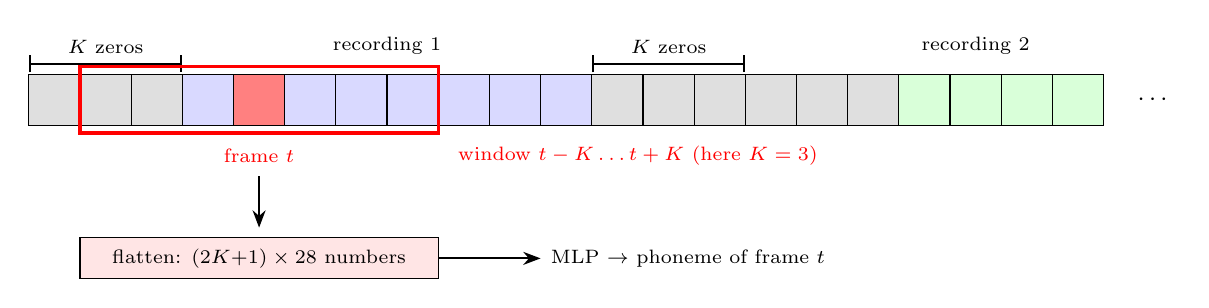
\begin{tikzpicture}[x=6.5mm,y=6.5mm]
  % padding + recording 1
  \foreach \i in {0,1,2} \draw[fill=gray!25] (\i,0) rectangle +(1,1);
  \foreach \i in {3,...,10} \draw[fill=blue!15] (\i,0) rectangle +(1,1);
  \foreach \i in {11,12,13} \draw[fill=gray!25] (\i,0) rectangle +(1,1);
  % recording 2
  \foreach \i in {14,15,16} \draw[fill=gray!25] (\i,0) rectangle +(1,1);
  \foreach \i in {17,...,20} \draw[fill=green!15] (\i,0) rectangle +(1,1);
  \node[font=\small] at (22,0.5) {$\cdots$};
  % labels
  \draw[|-|,thick] (0,1.2)--(3,1.2) node[midway,above,font=\scriptsize]{$K$ zeros};
  \node[font=\scriptsize,above] at (7,1.2) {recording 1};
  \draw[|-|,thick] (11,1.2)--(14,1.2) node[midway,above,font=\scriptsize]{$K$ zeros};
  \node[font=\scriptsize,above] at (18.5,1.2) {recording 2};
  % window around frame t
  \draw[red,very thick] (1,-0.15) rectangle (8,1.15);
  \draw[fill=red!50] (4,0) rectangle +(1,1);
  \node[font=\scriptsize,red] at (4.5,-0.6) {frame $t$};
  \node[font=\scriptsize,red,anchor=west] at (8.2,-0.6) {window $t-K \dots t+K$ (here $K=3$)};
  % flatten arrow
  \draw[arr] (4.5,-1.0) -- (4.5,-2.0);
  \draw[fill=red!10] (1,-3.0) rectangle (8,-2.2);
  \node[font=\scriptsize] at (4.5,-2.6) {flatten: $(2K{+}1)\times 28$ numbers};
  \draw[arr] (8,-2.6) -- (10,-2.6) node[right,font=\scriptsize]{MLP $\rightarrow$ phoneme of frame $t$};
\end{tikzpicture}
\caption{Context padding. Zeros (grey) separate the recordings. The network gets the window around
frame $t$ (red) and predicts the label of frame $t$ only.}
\label{fig:context}
\end{figure}

\subsection{Building batches on the GPU}
The whole padded training set ($\approx$1.9\,GB in float16) is kept \textbf{on the GPU}. A batch is
built with one indexing operation, without PyTorch's \texttt{DataLoader}. Multi-process loading is
unreliable inside Jupyter on Windows, and a single-process loader would make the GPU wait.

\begin{lstlisting}
def get_batch(data, idx):                      # idx: indices of the B frames in this batch
    offsets   = torch.arange(-K, K + 1)                    # (2K+1,)
    positions = centers[idx][:, None] + offsets[None, :]   # (B, 2K+1) frame positions
    x = padded[positions].reshape(len(idx), -1).float()    # (B, (2K+1)*28)
    return x, y[idx].long()
\end{lstlisting}

The data is shuffled every epoch with \texttt{torch.randperm}, and the batch size is 4096 frames
(8,812 batches per epoch).

\subsection{Model}\label{sec:model}
One configurable class, \texttt{PhonemeMLP}. Each hidden layer is the block
\textbf{Linear $\rightarrow$ BatchNorm $\rightarrow$ GELU $\rightarrow$ Dropout(0.2)}, and a final Linear
layer gives 40 \emph{logits} (one score per phoneme). No softmax is in the model because
\texttt{nn.CrossEntropyLoss} applies it internally.

\begin{figure}[H]
\centering
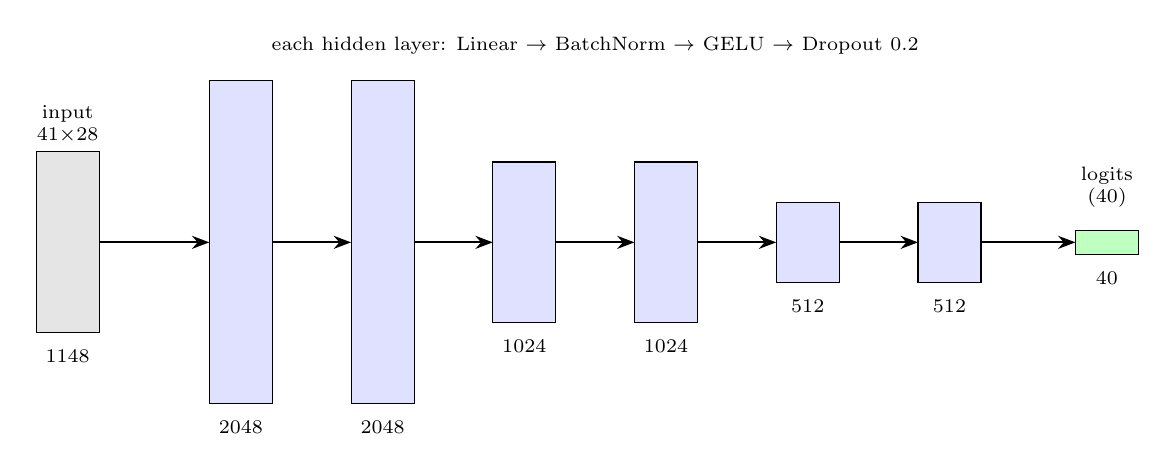
\begin{tikzpicture}[x=1mm,y=1mm]
  \foreach \x/\h/\lab/\n in {0/11.5/1148/in, 22/20.5/2048/a, 40/20.5/2048/b, 58/10.2/1024/c,
                              76/10.2/1024/d, 94/5.1/512/e, 112/5.1/512/f, 132/1.5/40/out} {
    \draw[fill=blue!12] (\x,-\h) rectangle (\x+8,\h);
    \node[font=\scriptsize] at (\x+4,-\h-3) {\lab};
  }
  \fill[gray!20] (0,-11.5) rectangle (8,11.5); \draw (0,-11.5) rectangle (8,11.5);
  \fill[green!25] (132,-1.5) rectangle (140,1.5); \draw (132,-1.5) rectangle (140,1.5);
  \foreach \a/\b in {8/22,30/40,48/58,66/76,84/94,102/112,120/132} \draw[arr] (\a,0)--(\b,0);
  \node[font=\scriptsize,align=center] at (4,15) {input\\41$\times$28};
  \node[font=\scriptsize] at (71,25) {each hidden layer: Linear $\rightarrow$ BatchNorm $\rightarrow$ GELU $\rightarrow$ Dropout 0.2};
  \node[font=\scriptsize,align=center] at (136,7) {logits\\(40)};
\end{tikzpicture}
\caption{The final ``pyramid'' MLP: 1148 inputs, hidden widths 2048-2048-1024-1024-512-512, 40 outputs.}
\end{figure}

\begin{table}[H]
\centering
\small
\begin{tabular}{lrrr}
\toprule
Layer & In $\rightarrow$ Out & Linear params & BatchNorm params \\
\midrule
Hidden 1 & 1148 $\rightarrow$ 2048 & 2,353,152 & 4,096 \\
Hidden 2 & 2048 $\rightarrow$ 2048 & 4,196,352 & 4,096 \\
Hidden 3 & 2048 $\rightarrow$ 1024 & 2,098,176 & 2,048 \\
Hidden 4 & 1024 $\rightarrow$ 1024 & 1,049,600 & 2,048 \\
Hidden 5 & 1024 $\rightarrow$ 512  &   524,800 & 1,024 \\
Hidden 6 & 512  $\rightarrow$ 512  &   262,656 & 1,024 \\
Output   & 512  $\rightarrow$ 40   &    20,520 & --- \\
\midrule
\multicolumn{2}{l}{\textbf{Total}} & \multicolumn{2}{r}{\textbf{10,519,592}} \\
\bottomrule
\end{tabular}
\caption{Parameter count (Linear: in$\times$out weights + out biases; BatchNorm: a scale and a shift per
neuron). The total is about half of the 20M limit.}
\end{table}

\textbf{Why a pyramid?} The first, widest layers can combine the 1148 inputs in many ways. The narrower
later layers compress this into features that separate the 40 classes. Most of the parameters sit in
the first two layers.

\subsection{Training setup}\label{sec:training}
\begin{itemize}\itemsep1pt
  \item \textbf{Loss:} cross-entropy, $\mathcal{L} = -\log \operatorname{softmax}(z)_{y}$ for logits $z$
        and true class $y$, averaged over the batch.
  \item \textbf{Optimiser:} AdamW, learning rate $10^{-3}$, weight decay $0.01$. AdamW is Adam with
        \emph{decoupled} weight decay, which gently pulls the weights towards zero (regularisation).
  \item \textbf{Learning-rate schedule:} cosine annealing over all epochs,
        $\eta_e = \tfrac{\eta_0}{2}\left(1+\cos\frac{\pi e}{E}\right)$: large steps at the start, very
        small steps at the end (from $10^{-3}$ down to $6\times10^{-6}$).
  \item \textbf{Mixed precision (AMP):} the forward pass runs in float16 where it is safe (about $2\times$
        faster). \texttt{GradScaler} scales the loss so that small gradients do not round to zero.
  \item \textbf{Model selection:} after each epoch the model is evaluated on dev, and the weights with the
        best dev accuracy are kept (\texttt{best.pt}).
  \item \textbf{Reproducibility:} fixed seed (42) for Python, NumPy and PyTorch.
\end{itemize}

\subsection{Sanity check: overfitting one batch}\label{sec:sanity}
Before any long training, a small model was trained for 300 steps on a single batch of 512 frames. It
reached \textbf{loss 0.0003 and 100\% accuracy}, which shows that the labels are aligned with the frames
and that the batching and training loop are correct. If a model cannot memorise one batch, there is a bug.

% ------------------------------------------------------------------ 5
\section{Ablation study}\label{sec:ablation}

Starting from a simple baseline, \textbf{one change is added at a time}, keeping all earlier changes. Every
step is trained for 3 epochs with the same seed and data, so the difference in dev accuracy shows the
effect of that one change.

\begin{table}[H]
\centering
\small
\setlength{\tabcolsep}{4pt}
\begin{tabular}{clrrrrr}
\toprule
Step & Change & Params & Train & Dev & Gain & Min/ep. \\
\midrule
1 & Baseline: $K{=}5$, 2$\times$512, ReLU, Adam & 0.44M & 70.07 & 68.06 & ---  & 0.3 \\
2 & + CMVN                                  & 0.44M & 72.46 & 71.36 & +3.30 & 0.3 \\
3 & + context $K{=}20$ (41 frames)          & 0.87M & 76.70 & 75.24 & +3.88 & 0.3 \\
4 & + pyramid 2048$\rightarrow$512 + BatchNorm & 10.5M & 87.05 & 81.28 & \textbf{+6.04} & 3.1 \\
5 & + Dropout 0.2                           & 10.5M & 80.73 & 81.74 & +0.46 & 3.3 \\
6 & + GELU instead of ReLU                  & 10.5M & 82.41 & 82.55 & +0.81 & 3.3 \\
7 & + AdamW + cosine schedule               & 10.5M & 83.18 & 82.90 & +0.35 & 3.4 \\
\bottomrule
\end{tabular}
\caption{Ablation results. Train = train accuracy (\%) in epoch 3; Dev = best dev accuracy (\%) of the 3
epochs; Gain = change in dev accuracy from the previous step. Total gain: +14.84 points.}
\label{tab:ablation}
\end{table}

\begin{figure}[H]
\centering
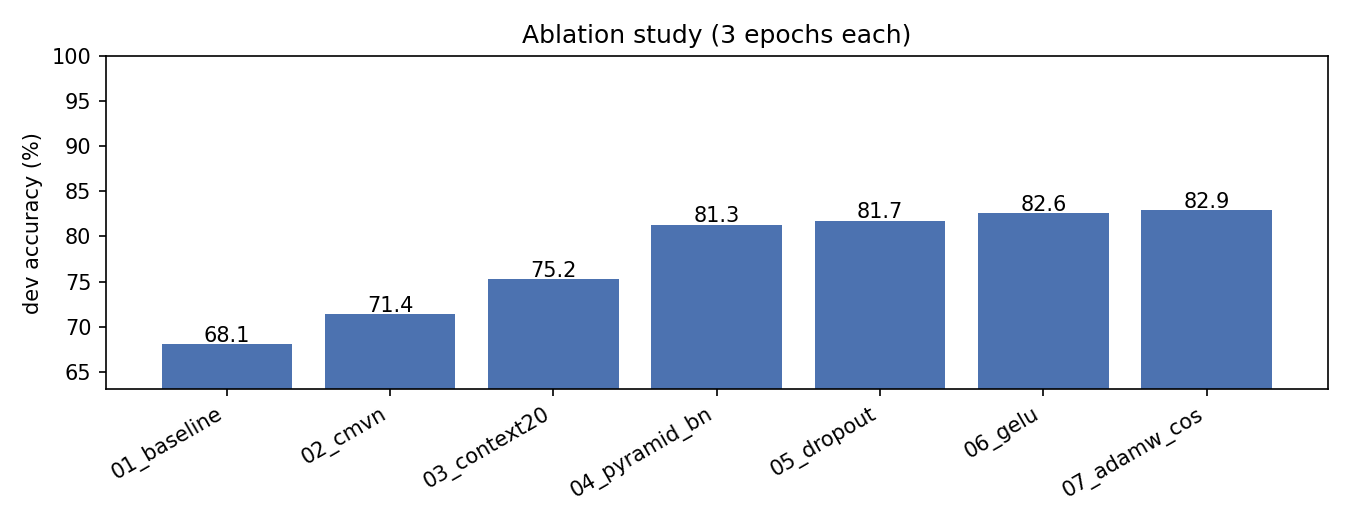
\includegraphics[width=0.8\textwidth]{figures/ablation.png}
\caption{Dev accuracy after each ablation step (3 epochs each).}
\end{figure}

\textbf{What each step shows}
\begin{enumerate}\itemsep1pt
  \item \textbf{Baseline (68.06\%).} Already four times better than always predicting \texttt{[SIL]}
        (16.6\%), so the inputs carry a lot of information.
  \item \textbf{CMVN (+3.3).} Removing speaker and microphone offsets makes the same phoneme look more
        alike across recordings.
  \item \textbf{Context $K{=}20$ (+3.9).} Phonemes last several frames and depend on their neighbours, so
        a longer window helps. The input grows from 308 to 1148 numbers, but the model only grows from
        0.44M to 0.87M parameters.
  \item \textbf{Pyramid + BatchNorm (+6.0, the largest gain).} The small model was too small to use all the
        context (\emph{underfitting}). With 10.5M parameters it can learn much richer features, and
        BatchNorm keeps such a deep network stable. However, this step started to \textbf{overfit}: train
        accuracy jumped to 87.05\% while dev stayed at 81.28\%, and the dev loss rose from 0.578 (epoch 2)
        to 0.596 (epoch 3).
  \item \textbf{Dropout (+0.5).} Fixes that overfitting: dev loss falls to 0.545 and keeps decreasing.
        Train accuracy now looks \emph{lower} than dev, because it is measured during training with
        dropout switched on, while dev is evaluated with the full network.
  \item \textbf{GELU (+0.8).} A smooth version of ReLU: negative inputs give small non-zero outputs, so
        gradients do not stop completely, which slightly improves learning.
  \item \textbf{AdamW + cosine (+0.35).} The gain is small in 3 epochs, but these two matter more in a
        long run. The falling learning rate lets the model settle into a good minimum, and weight decay
        limits overfitting over many epochs.
\end{enumerate}

\textbf{Why an ablation study and not one large run?} A single large run would give the same final
score, but it would not show \emph{why} each component is there. The ablation measures every choice,
shows where the big gains come from (model size, context and normalisation, not the activation
function), and revealed the overfitting that justified dropout. Short 3-epoch runs keep it affordable
(about 42 minutes in total).

% ------------------------------------------------------------------ 6
\section{Final model}\label{sec:final}

The configuration of step 7 was trained for \textbf{20 epochs}, with the cosine schedule stretched over
the 20 epochs. Each epoch took 3.4 minutes (67.6 minutes in total).

\begin{table}[H]
\centering
\small
\begin{tabular}{ll}
\toprule
Setting & Value \\
\midrule
Context & $K=20$ (41 frames, 1148 inputs), CMVN per recording \\
Hidden layers & 2048, 2048, 1024, 1024, 512, 512 with BatchNorm, GELU, Dropout 0.2 \\
Parameters & 10,519,592 \\
Optimiser & AdamW, lr $10^{-3}$, weight decay 0.01, cosine schedule over 20 epochs \\
Batch size / precision & 4096 frames / mixed precision (float16) \\
\bottomrule
\end{tabular}
\caption{Final configuration.}
\end{table}

\begin{table}[H]
\centering
\small
\begin{tabular}{rcrrrr}
\toprule
Epoch & Learning rate & Train loss & Train acc (\%) & Dev loss & Dev acc (\%) \\
\midrule
 1 & $1.00\times10^{-3}$ & 0.760 & 75.46 & 0.593 & 80.18 \\
 5 & $9.05\times10^{-4}$ & 0.484 & 83.58 & 0.500 & 83.17 \\
10 & $5.78\times10^{-4}$ & 0.431 & 85.17 & 0.480 & 83.96 \\
15 & $2.06\times10^{-4}$ & 0.394 & 86.26 & 0.472 & 84.40 \\
19 & $2.45\times10^{-5}$ & 0.378 & 86.77 & 0.471 & \textbf{84.55} \\
20 & $6.16\times10^{-6}$ & 0.377 & 86.81 & 0.471 & 84.55 \\
\bottomrule
\end{tabular}
\caption{Selected epochs of the final training (all 20 are in the notebook and in
\texttt{runs/final/history.csv}).}
\end{table}

\begin{figure}[H]
\centering
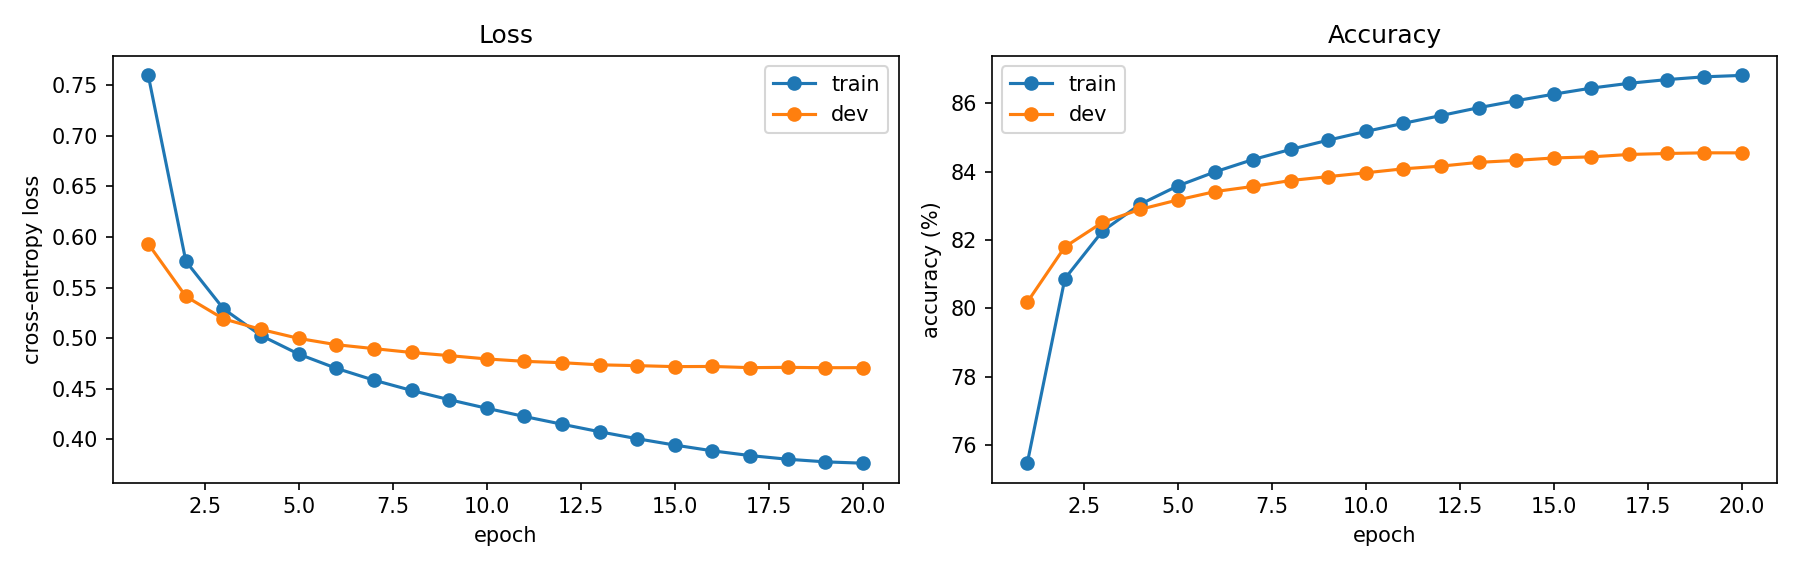
\includegraphics[width=0.95\textwidth]{figures/learning_curves.png}
\caption{Learning curves of the final model: loss (left) and accuracy (right) for train and dev.}
\end{figure}

\textbf{Reading the curves.}
\begin{itemize}\itemsep1pt
  \item Dev accuracy rises every epoch and levels off after about epoch 17, when the learning rate is very
        small. More epochs at this setting would add little.
  \item The dev loss never rises, so the final model does \textbf{not overfit} badly. The final train/dev gap
        is only 2.3 points (86.81\% vs 84.55\%), thanks to dropout, weight decay and the very large
        training set (36M frames).
  \item The long run adds \textbf{+1.65 points} over the 3-epoch ablation version (82.90\% $\rightarrow$
        84.55\%). This is where AdamW and the cosine schedule pay off.
  \item The best weights (epoch 19) are used for the test predictions.
\end{itemize}

% ------------------------------------------------------------------ 7
\section{Error analysis}\label{sec:errors}

\begin{figure}[H]
\centering
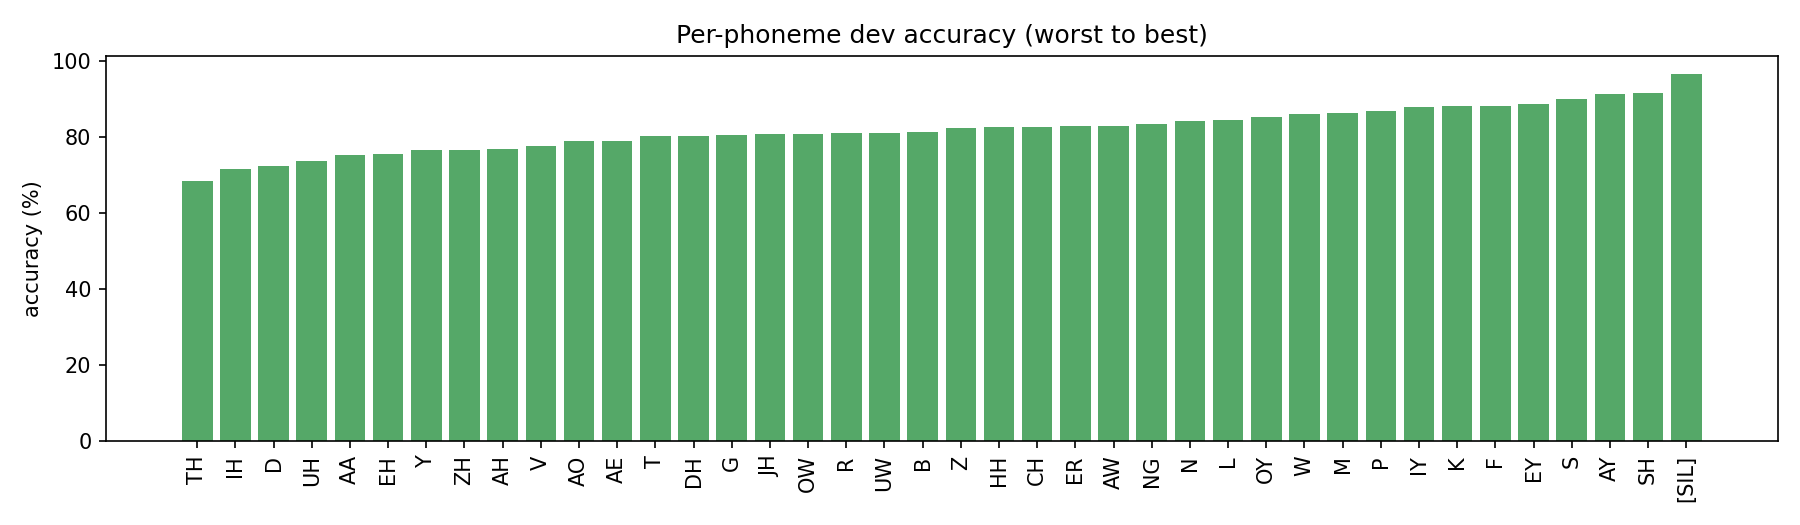
\includegraphics[width=0.95\textwidth]{figures/per_class_acc.png}
\caption{Dev accuracy for each phoneme, from worst to best.}
\end{figure}

\begin{itemize}\itemsep1pt
  \item \textbf{Easiest:} \texttt{[SIL]} 96.6\%, \texttt{SH} 91.7\%, \texttt{AY} 91.4\%, \texttt{S} 90.2\%.
        These are long or acoustically distinctive sounds.
  \item \textbf{Hardest:} \texttt{TH} 68.4\%, \texttt{IH} 71.7\%, \texttt{D} 72.4\%, \texttt{UH} 73.6\%.
        These are short, weak or easily confused sounds.
\end{itemize}

\begin{figure}[H]
\centering
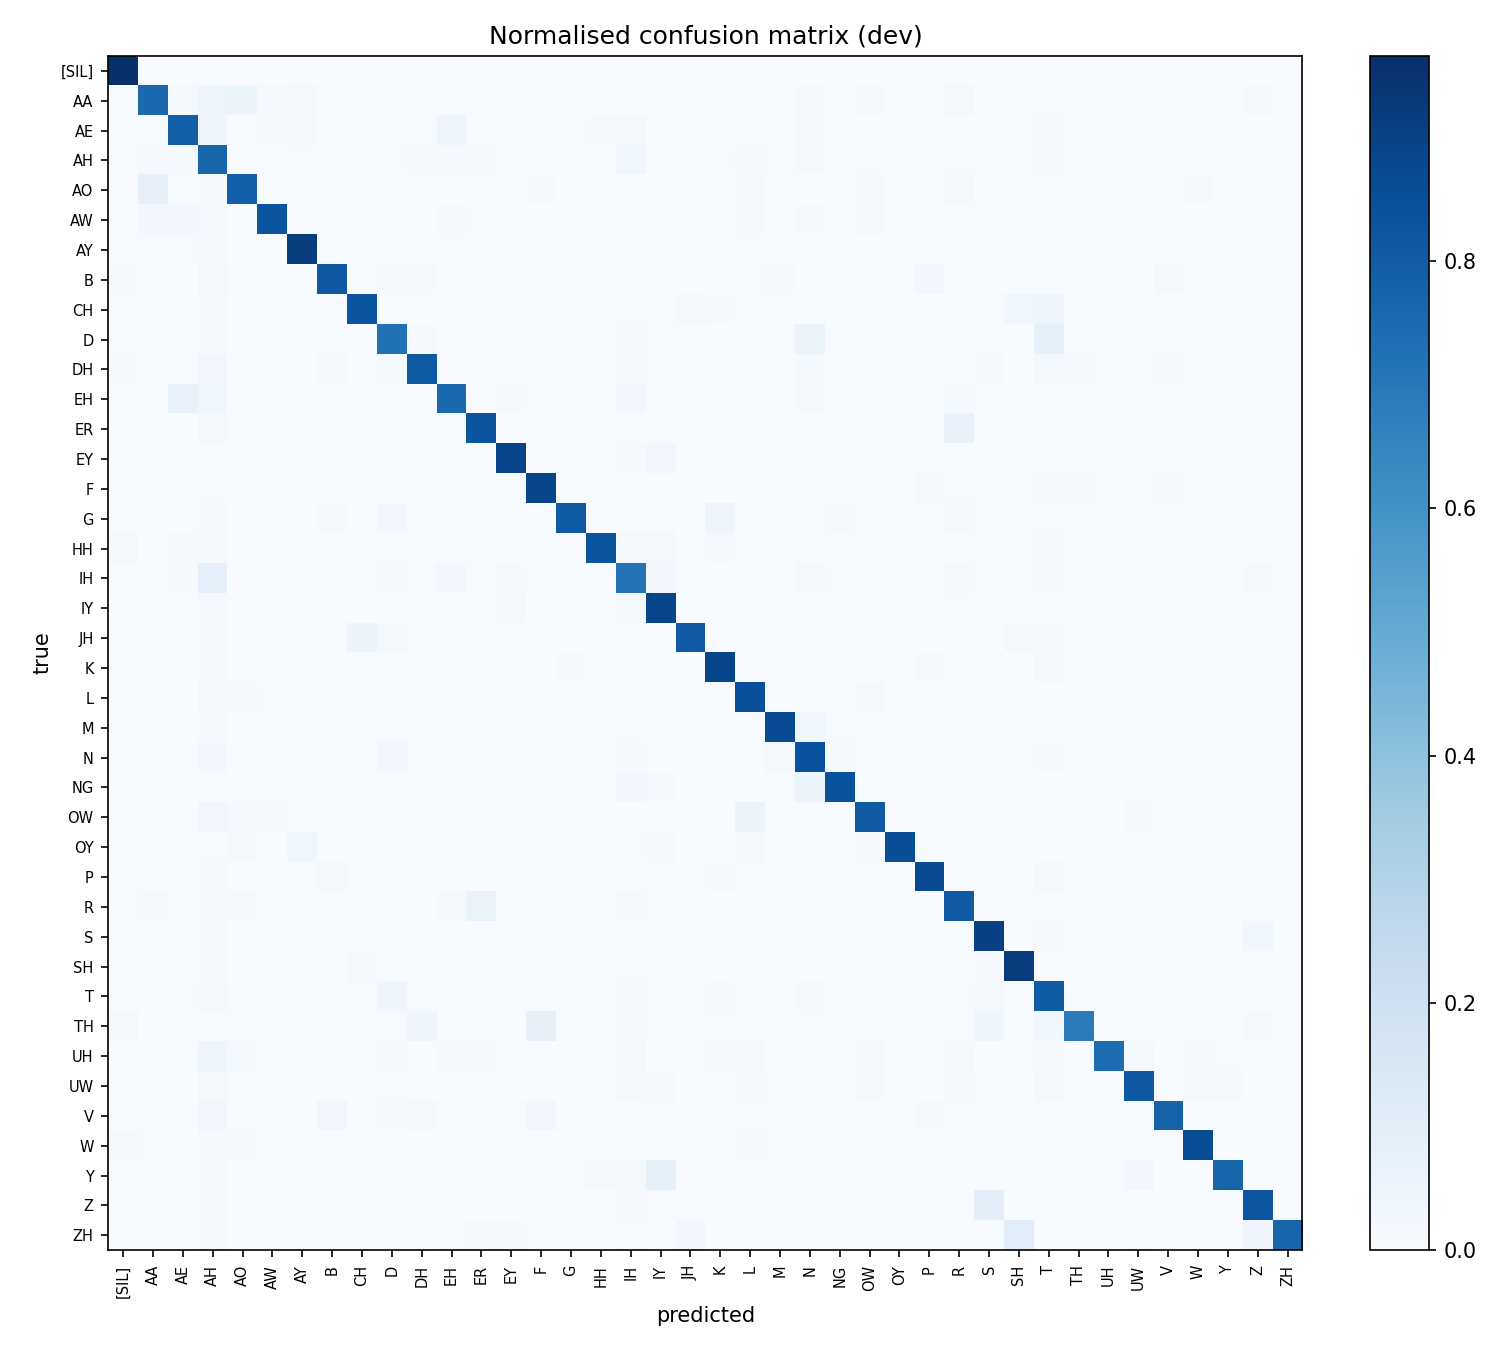
\includegraphics[width=0.62\textwidth]{figures/confusion_matrix.png}
\caption{Normalised confusion matrix on dev (row = true phoneme, column = predicted). The strong diagonal
means most frames are correct.}
\end{figure}

\begin{table}[H]
\centering
\small
\begin{tabular}{llrl}
\toprule
True & Predicted as & \% of true class & Why they are similar \\
\midrule
ZH & SH & 10.5 & same place of articulation, only voicing differs \\
Z  & S  &  9.2 & voiced vs.\ unvoiced pair \\
IH & AH &  8.7 & short, unstressed vowels \\
Y  & IY &  8.3 & \texttt{Y} is a glide that sounds like \texttt{IY} \\
D  & T  &  7.9 & voiced vs.\ unvoiced pair \\
TH & F  &  7.6 & both weak, noise-like fricatives \\
AO & AA &  7.5 & neighbouring back vowels \\
EH & AE &  6.9 & neighbouring front vowels \\
ER & R  &  6.6 & \texttt{ER} is an \texttt{R}-coloured vowel \\
R  & ER &  6.3 & (same pair, other direction) \\
\bottomrule
\end{tabular}
\caption{The ten most frequent confusions on dev.}
\end{table}

The mistakes are \textbf{linguistically sensible}: almost all of them are between phonemes that differ in
one feature only (often voicing) or that are neighbouring vowels. The model is not guessing randomly;
it confuses sounds that people also find similar.

% ------------------------------------------------------------------ 8
\section{Test predictions and submission}
The test set is processed exactly like dev: the same CMVN, the same $K=20$ padding, and files in sorted
order. The best model (epoch 19) then predicts one phoneme per frame. \texttt{submission.csv} has one row
per test frame, with the columns \texttt{id} (running frame number) and \texttt{label} (the phoneme
string). It was checked before submission:
\begin{itemize}\itemsep0pt
  \item 1,934,138 rows, exactly one per test frame, with no missing values;
  \item ids run from 0 to 1,934,137 in order;
  \item every label is one of the 40 valid classes, and all 40 appear;
  \item the share of each predicted phoneme matches its share in train within 1.3 percentage points
        (e.g.\ \texttt{[SIL]} 16.0\% predicted vs.\ 17.3\% in train), so the model is not collapsing
        onto one class.
\end{itemize}
Test labels are hidden, so the dev accuracy of 84.55\% is our estimate of the test accuracy. Dev and
test come from the same kind of recordings (``clean'' LibriSpeech).

% ------------------------------------------------------------------ 9
\section{Notebook documentation}

The notebook \texttt{Yassin\_120230122.ipynb} runs top to bottom with \textbf{Run All}. Every section
starts with a short explanation cell.

\begin{table}[H]
\centering
\small
\begin{tabular}{rp{3.6cm}p{9.6cm}}
\toprule
\# & Section & What it does \\
\midrule
0  & GPU check, configuration & Prints the PyTorch/CUDA versions and GPU memory, runs a test matrix
                                multiplication, and stops if there is no GPU. All settings (paths,
                                batch size 4096, seed 42, \texttt{DEBUG}) are in one cell. \\
1  & Data loading, exploration & \texttt{load\_split} reads or caches each split. Plots one recording's
                                MFCCs and the class distribution. \\
2  & Pre-processing & \texttt{build\_padded}: CMVN and $K$ zero frames around each recording, plus the
                                \texttt{centers} index; the result is moved to the GPU. \\
3  & Batching & \texttt{get\_batch} gathers the $(2K{+}1)$-frame windows; a shape check confirms 308
                                inputs for $K=5$. \\
4  & Model & \texttt{PhonemeMLP}, with configurable widths, BatchNorm, dropout and activation; prints the final
                                architecture and asserts fewer than 20M parameters. \\
5  & Training functions & \texttt{train\_one\_epoch} (AMP, progress bar with time left),
                                \texttt{evaluate}, \texttt{predict}, and \texttt{run\_experiment} (optimiser,
                                scheduler, saving, ETA). \\
6  & Sanity check & Overfits one batch (100\%). \\
7  & Ablation study & Runs the 7 steps; writes \texttt{results/ablation.csv} and the bar chart. \\
8  & Final training & 20 epochs of the step-7 configuration. \\
9  & Analysis & Learning curves, per-phoneme accuracy, confusion matrix, top confusions. \\
10 & Submission & Predicts the test set and writes \texttt{submission.csv} and \texttt{results/summary.json}. \\
\bottomrule
\end{tabular}
\caption{Notebook sections.}
\end{table}

\textbf{Project folders.}
\begin{itemize}\itemsep1pt
  \item \texttt{cache/}: the merged data (train 1.96\,GB, dev and test about 0.1\,GB each). It is built
        once (about 10 minutes from disk) and then loads in seconds.
  \item \texttt{runs/<run\_name>/}: one folder per training run (\texttt{01\_baseline} \dots\
        \texttt{07\_adamw\_cos}, \texttt{final}), each with \texttt{config.json} (settings),
        \texttt{history.csv} (loss, accuracy, learning rate and time per epoch), \texttt{best.pt} (best dev
        weights) and \texttt{epochs/epoch\_XX.pt} (weights after every epoch).
  \item \texttt{results/}: all figures, plus the tables of the ablation, the per-phoneme accuracy and the
        top confusions (\texttt{.csv}) and the final summary (\texttt{summary.json}).
\end{itemize}

\textbf{Restarting safely.} A run whose \texttt{history.csv} already has all its epochs is \emph{not}
retrained: its weights are loaded and its saved training log is printed again. Re-running the whole
notebook therefore takes about 5 minutes instead of about 2 hours, and gives the same results and the
same \texttt{submission.csv}. Setting \texttt{RETRAIN = True} forces training from scratch.

\textbf{Progress and time estimates.} Each run shows an overall bar (epochs done, \textbf{ETA} for the
run) and a per-epoch bar (batches done, \textbf{time left in the epoch}, running loss and accuracy), and
prints one summary line per epoch.

% ------------------------------------------------------------------ 10
\section{Design choices and limitations}

\begin{table}[H]
\centering
\small
\begin{tabular}{p{4.2cm}p{11cm}}
\toprule
Choice & Reason \\
\midrule
MLP on a context window & Required by the assignment; the context window gives the MLP the temporal
                          information that a sequence model would otherwise provide. \\
$K=20$ & Clear gain over $K=5$ (+3.9). Larger windows grow the input and memory further. \\
CMVN per recording & Removes speaker and microphone effects; costs nothing at test time. \\
float16 storage, data on the GPU & Fits the 36M training frames in the 6\,GB GPU and 16\,GB RAM, and
                          makes batching fast. \\
No \texttt{DataLoader} & Multi-process loading is unreliable in Jupyter on Windows; GPU indexing is
                          simpler and faster here. \\
Batch size 4096 & Uses the GPU well; BatchNorm statistics are very stable with large batches. \\
Mixed precision & About 2$\times$ faster training at no loss in accuracy. \\
Dev set for selection & Test labels are hidden; dev chooses the settings and the best epoch, and the test
                          set is used only once, for the final predictions. \\
\bottomrule
\end{tabular}
\caption{Main design choices.}
\end{table}

\textbf{Limitations and possible improvements.} Each ablation step is a single 3-epoch run with one seed,
so the small gains (under 1 point) are within run-to-run noise; the large gains (CMVN, context, model
size) are clearly real. Within the MLP setting, further gains could come from a larger context, more
epochs, frequency/time masking as data augmentation, or averaging several models, all at the cost of more
training time and complexity.

% ------------------------------------------------------------------ 11
\section{Conclusion}

A frame-level phoneme classifier was built from a plain MLP and improved step by step. The ablation study
showed that the biggest improvements came from \textbf{model capacity with BatchNorm} (+6.0 points),
\textbf{a wider context window} (+3.9) and \textbf{per-recording normalisation} (+3.3). Dropout, GELU,
AdamW and the cosine schedule then added smaller gains and stopped the large model from overfitting. The
final 10.5M-parameter model reaches \textbf{84.55\% dev accuracy}, compared with 68.06\% for the baseline
and 16.6\% for always predicting silence, with a small 2.3-point gap between train and dev accuracy. Its
remaining errors are mostly between phonemes that sound alike, such as \texttt{Z}/\texttt{S} and
\texttt{D}/\texttt{T}. The code stays simple (one model class, one training loop), every result is saved
per run, and the notebook reproduces the submission with one \textbf{Run All}.

\end{document}
